% Written by Louise Fussien

% This file CAN NOT be compiled on its own
% It is included by ../Book_of_Specifications.tex

\subsection{Analyse et progrès}

\subsubsection{Status actuel}

Depuis le début de notre projet, nous avons effectué une analyse approfondie de nos objectifs et des tâches à accomplir. 
L'acte un a été entièrement créé avec succès, ce qui représente une étape majeure dans l'avancement de notre projet.

\subsubsection{Délais rencontrés et raisons}

Toutefois, notre progression a été marquée par des défis imprévus. 
Deux membres clés de notre équipe ont quitté le projet, ce qui a significativement impacté notre capacité de travail. 
Bien que l'administration ait ajouté un nouveau membre à notre groupe, cela n'a pas suffi à compenser entièrement la perte de compétences et d'expérience des membres sortants.
\\


Les délais que nous avons rencontrés sont principalement dus à ces départs inattendus. 
L'intégration du nouveau membre a pris du temps, non seulement pour qu'il se familiarise avec le projet, mais aussi pour qu'il soit pleinement opérationnel. De plus, notre ambition de perfectionnisme a joué un rôle important. 
Nous avons été très méticuleux dans chaque étape du développement, ce qui, bien que bénéfique pour la qualité du projet, nous a obligé à raccourcir le nombre d'actes prévus initialement.
\subsection{Organisation du groupe}

\subsubsection{Communication}

Pour assurer une collaboration efficace au sein de notre groupe de projet, nous avons opté pour l'utilisation de plusieurs outils de communication. 
Principalement, nous avons utilisé Discord, une plateforme de communication instantanée, pour faciliter les échanges en temps réel entre les membres du groupe. 
Discord nous a permis de maintenir une communication fluide et réactive, essentielle pour coordonner nos efforts et résoudre rapidement les problèmes rencontrés pendant le développement du projet. 
Les fonctionnalités de chat vocal et textuel de Discord ont été particulièrement utiles pour organiser des réunions spontanées et des discussions en groupe, améliorant ainsi notre efficacité collaborative.
\\

En complément de Discord, nous avons également profité des sessions de travail en groupe en présentiel à l'EPITA. Ces rencontres physiques nous ont offert l'opportunité de discuter en profondeur des aspects techniques et conceptuels du projet, de partager des idées de manière plus interactive et de travailler sur des tâches spécifiques ensemble. Cette combinaison d'interaction en ligne via Discord et en personne à l'université nous a permis de tirer parti des avantages uniques de chaque mode de communication,
renforçant ainsi notre cohésion d'équipe et notre efficacité dans l'accomplissement des objectifs du projet.
\\



\subsubsection{GitHub}

Github a joué un rôle central dans la gestion et le partage de notre code source tout au long du projet.
Nous avons utilisé GitHub comme plateforme principale pour héberger notre repository de projet, ce qui nous a permis de collaborer efficacement sur le code.
Chaque membre du groupe a pu créer des branches de développement distinctes pour travailler sur des fonctionnalités spécifiques sans perturber la branche principale, tout en utilisant des pull requests pour fusionner les contributions et effectuer des révisions par les pairs.
\\

L'intégration de GitHub avec notre flux de travail nous a offert plusieurs avantages.
Premièrement, cela a facilité la gestion des versions du code et le suivi des modifications apportées à mesure que le projet évoluait.
Deuxièmement, GitHub a facilité la détection et la résolution des conflits de fusion, assurant ainsi l'intégrité du code source partagé entre les membres du groupe.
\\
\subsubsection{Répartition des tâches }


La répartition des charges au sein de notre équipe a été stratégique et s'est adaptée aux défis que nous avons rencontrés tout au long du projet.
Initialement, chaque membre de l'équipe s'est vu attribuer des responsabilités spécifiques en fonction de ses compétences et de son expertise, telles que définies dans le cahier des charges technique initial.
\\

Cependant, notre progression a été marquée par des changements significatifs.
Nous avons dû faire face au départ inattendu de deux membres clés de l'équipe.
Cela a eu un impact direct sur notre capacité à respecter les délais et à maintenir la cohésion au sein du groupe. Pour pallier ces départs, sans recruter de nouvelles personnes, l'administration a intégré un nouveau membre existant dans notre groupe.
\\

Cette transition n'a pas été sans défis.
L'intégration du nouveau membre a demandé du temps pour s'adapter aux dynamiques de l'équipe et pour assimiler les responsabilités en cours.
Malgré ces ajustements, nous avons maintenu une communication ouverte et des réunions régulières pour aligner les attentes et assurer une collaboration harmonieuse.
\\

Au fur et à mesure que nous nous sommes adaptés à ces changements,
nous avons également mis à jour notre cahier des charges technique pour refléter les nouvelles répartitions et les ajustements nécessaires.
Chaque nouvelle itération du cahier technique a intégré les modifications stratégiques et les décisions prises en réponse aux défis rencontrés,y compris la redistribution des tâches et des responsabilités entre les membres existants.
\\

\subsubsection{Cahier des charges techniques}
Pendant le développement du projet, nous avons élaboré plusieurs versions du cahier technique pour répondre aux évolutions et aux défis rencontrés.
Chaque itération a été cruciale pour ajuster notre approche et nos spécifications en fonction des besoins changeants du projet.
\\

Initialement, notre cahier technique définissait les fondations et les objectifs techniques de notre jeu.
Nous avons spécifié les fonctionnalités essentielles, l'architecture logicielle prévue, ainsi que les technologies clés à utiliser.
Cette première version nous a permis de commencer le développement sur des bases solides.
\\

Le dernier cahier des charges technique, intégré dans ce rapport final, reflète ces ajustements. Il décrit non seulement les spécifications finales du jeu telles qu'elles ont évolué tout au long du processus, mais aussi les décisions stratégiques prises pour surmonter les défis rencontrés.


\subsubsection{Cahier des charges techniques}
% This file CAN NOT be compiled on its own
% It is included by ../Book_of_Specifications.tex

% TODO Update the technical book

Les deux prochaines pages sont dédiées au cahier des charges technique.
Ce document détaille les contraintes et les caractéristiques techniques nécessaires pour répondre aux besoins du projet.
Il synthétise toutes les réponses aux questions techniques que l'on peut se poser sur le projet.
\\

Le cahier des charges technique est divisé en deux parties.
La première partie détaille les spécificités du jeu et les choix techniques qui ont été réalisés. 
La deuxième partie donne des informations sur la repartition des tâches et leur avancement.
\\

Des changements ont été apportés au cahier des charges technique depuis sa dernière version.
Le nom du jeu a été modifié, le départ de Mohamed Aziz et Alexandre a été pris en compte, et des changements ont été apportés au diagramme de Gantt pour refléter l'avancé du projet.
\\

Le dernier cahier des charges technique, intégré dans ce rapport final, reflète ces ajustements. Il décrit non seulement 
les spécifications finales du jeu telles qu'elles ont évolué tout au long du processus, mais aussi les décisions stratégiques prises pour surmonter les défis rencontrés.



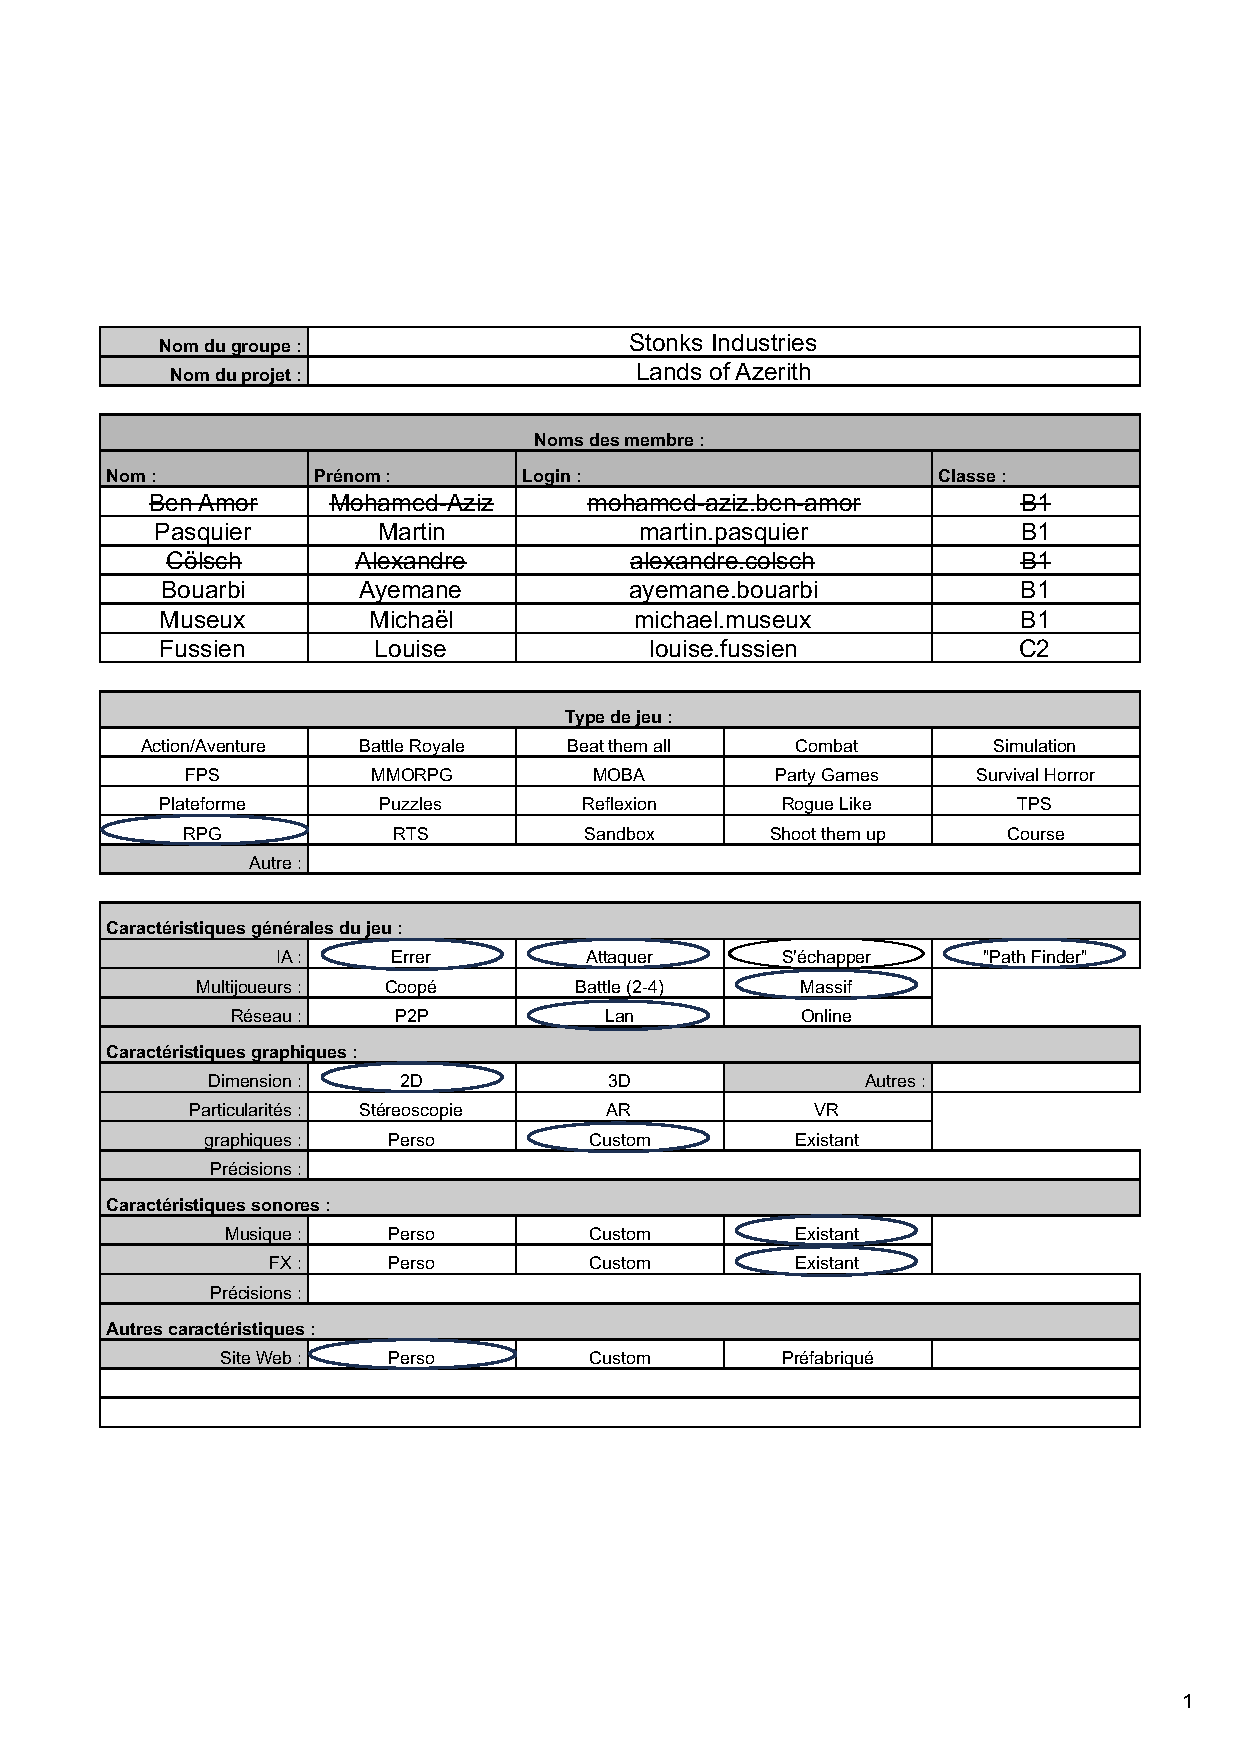
\includepdf[pages=1]{technical_book/page-1.pdf}

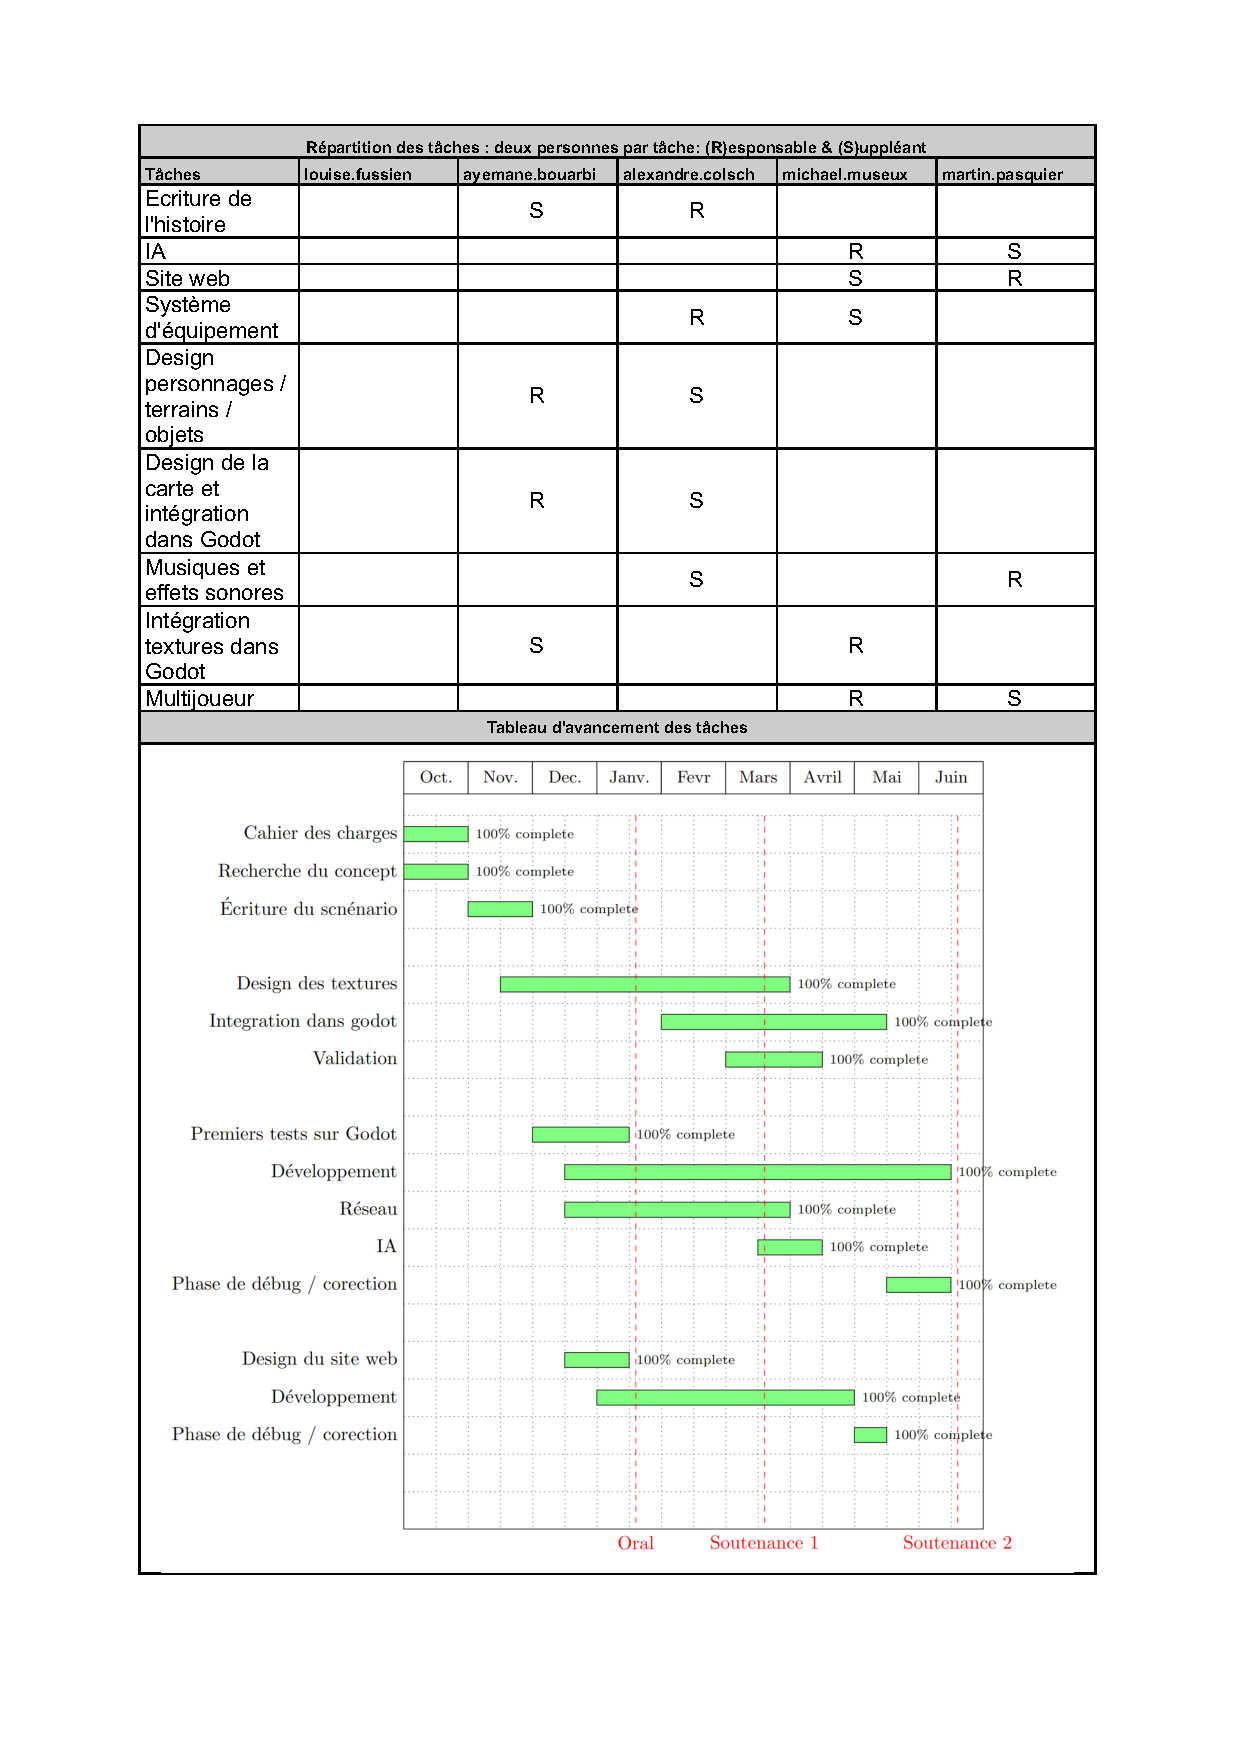
\includepdf[pages=1]{technical_book/page-2.pdf}

